\chapter{Graph Tracking in Probabilistic Models}
\label{cha:graph-track-prob}

The system described in chapter~\ref{cha:impl-dynam-graph}, implemented in a Julia package
\irtrackerjl{}, can now be utilized for the analysis of probabilistic models written in \dppljl{},
and for posterior inference in \turingjl{}.  This part of the work is realized in another package,
\autogibbsjl{}, which is available as open-source
code\footnote{\url{https://github.com/phipsgabler/AutoGibbs.jl}}.  There are two applications
provided, built on top of the graph tracking functionality: first, dependency analysis of random
variables in a model can be performed.  This results in the complete graphical model for static
models, and a slice of it for dynamic models.  The resulting graph can be plotted for visualization.
Second, given the dependency graph, the conditional likelihoods of unobserved variables in static
models can be extracted.  With these, analytic Gibbs conditionals can be derived and used in
\turingjl{}'s within-Gibbs sampler.

\section{Dependency Analysis in Dynamic Models}
\label{sec:dependency-analysis}

In order to use \irtrackerjl{} to extract the dependencies in a probabilistic model written in
\dppljl{}, we need to remember the structure of such models, which was introduced in
section~\ref{sec:prob-prog}: there is one evaluator function, into which the original code is
transformed, and which evaluates the model in different modes.  This function has the same structure
as the original code, but adds some more complicated book-keeping logic to it, and transforms the
tilde statements into function calls with some additional metadata.  Furthermore, when calling the
model as a callable object, there are several layers of dispatch (about five layers of nesting,
depending on the arguments), until the real evaluator function is actually hit.  On the other hand,
there is no further nesting involved beyond the evaluator function~-- \turingjl{} simply does not
support nested models, for technical reasons.

Therefore, we at first need to introduce an \irtrackerjl{} context that will record all the internal
function calls down to the evaluator function, and stop there.  Similar to the
\jlinl{DepthLimitContext} demonstrated on page~\pageref{lst:depthlimitcontext}, the main task here
is to overload the \jlinl{canrecur} method to stop at the right call.  This can easily be done by
introducing a helper predicate function \jlinl{ismodelcall} that dispatches on the involved types.
Next, we notice that the resulting computation graph consists of a nested and quite unusable
structure, due to the initial levels of nesting.  To work with the model code, we need to strip the
outer layers off the inner node containing the trace of the evaluator function.  Thirdly, many of
the statements in the trace of the evaluator function do not have relevance for dependency
analysis~-- like those that stem from internal calculations done by the model, or statements that
were written by the user but to not lie on the dependency graph, such as debugging statements or the
lowered code of for loops, in some cases.  These we can strip off in advance, so as to clean the raw
dependency trace.  These three preparation steps are put together in one method:
\begin{lstlisting}
function slicedependencies(model::Model{F}, args...) where {F}
    trace = trackmodel(model, args...)
    strip = strip_model_layers(F, trace)
    slice = strip_dependencies(strip)
    return slice
end
\end{lstlisting}
Here, \jlinl{trackmodel} extracts the computation graph with the context for models tracking,
\jlinl{strip_model_layers} removes the outer method calls, and \jlinl{strip_dependencies} removes
all SSA code that is not on the dependency graph spanned by the sampling statements.

The final and most intricate step is to add all the remaining SSA statements to a new graph
structure, that describes a more domain-specific representation.  In this \jlinl{Graph} type, only
assumption, observation, call, and constant nodes remain, containing relevant metadata such as their
values, variable names, and distribution objects.  In addition, the object stores intermediate
information used during its construction, such as the mapping between newly generated and original
references.  The graph construction is implemented in a function \jlinl{makegraph}, and we finally
have one exported function
\begin{lstlisting}
function trackdependencies(model, args...)
    slice = slicedependencies(model, args...)
    return makegraph(slice)
end
\end{lstlisting}
There are two complications regarding \jlinl{makegraph}.  For one, model arguments are handled
specially by \dppljl{}~-- there are some internal arguments added, and the original arguments are
inspected to allow to run the same model in generative or posterior mode.  This part needs to be
sorted out, so that the passed argument values are correctly set up as constants in the dependency
graph, but since all information is present, the task is resolved by correctly identifying the
arguments and restructuring their contents into the right form.

The other problem is the handling of mutation, and tracking of modified array elements.  For
example, a hidden Markov model might contain code like this:
\begin{lstlisting}
s = zeros(Int, N)
s[1] ~ Categorical(K)
for i = 2:N
    s[i] ~ Categorical(T[s[i-1]])
end
\end{lstlisting}
In order to express the dependency between successive elements of \jlinl{s}, an empty array is first
set up, and then subsequently populated by the results of the tilde statements describing the Markov
process.  In this form, only the individual variables \jlinl{s[i]} are recognized by the model
language.  Internally, the tilde statements are translated to array assignments of the form
\jlinl{s[i] = tilde_assume(...)}, but with additional lowering of the involved arguments, after
which the corresponding IR will look approximately like this:
\begin{lstlisting}
%9 = %i - 1                                  # i - 1
%10 = getindex(%s, %9)                       # s[i - 1]
%11 = getindex(%T, %10)                      # T[s[i - 1]]
%12 = VarInfo{:s}(((%i,),))
%13 = Categorical(%11)
%14 = tilde_assume(..., %13, ..., %12, ...)  # %14 ~ %13
%15 = setindex!(%s, %14)                     # s[i] = %14
\end{lstlisting}
(to be understood symbolically, not as real SSA~-- several statements have been collapsed).  We see
that the direct association between the variable \jlinl{s} is not preserved in the line of the tilde
method, but spread over multiple statements. Even worse, since all statements for the different
\jlinl{s[i]} result in mutations of \jlinl{\%s}, the immediate dependency between \jlinl{s[i]} and
\jlinl{s[i-1]} is not available structurally, but must be recovered dynamically.

The \jlinl{makegraph} implementation solves this by successively identifying mutated arrays
representing random variables by inspecting the indexing calls around tilde statements, and storing
the association between the assumption and the array elements.  This part of the procedure is the
most intricate one, and not complete; there may exist cases where mutation is able to
\enquote{circumvent} the dependency analysis.  Additionally, the matching between indexing arguments
involves some careful treatment of variable names; the existing \dppljl{} API for this functionality
is not very comprehensive.  Due to this, the current implementation of \autogibbsjl{} currently only
supports \enquote{simple} indexing by one tuple of integers.  Other, more general indexing styles
allowed in Julia could be added in future extensions.  Furthermore, broadcasting tilde statements,
that are supported in \dppljl{}, are not supported by \autogibbsjl{} either.

\newthought{As an example} for the resulting graphs, take the two simple models in
listing~\ref{lst:dependency-examples}.  The pretty-printed dependency \jlinl{Graph} objects
extracted from them are shown in listing~\ref{lst:trace-examples} below.  We can see that the model
arguments for observations occur as constant values, and all of the intermediate transformation
visible in the original model definitions are observed.  From this structure, \autogibbsjl{} can
construct output in the Dot graph format and visualized using GraphViz \parencite{gansner2000open}.
The visual outputs of the example models is shown in figure~\ref{fig:geom-deps}.

\begin{lstfloat}[p]
\begin{lstlisting}[style=lstfloat]
@model function bernoulli_mixture(x)
    w ~ Dirichlet(2, 1/2)
    π ~ DiscreteNonParametric([0.3, 0.7], w)
    x ~ Bernoulli(π)
end

@model function hierarchical_gaussian(x)
    λ ~ Gamma(2.0, inv(3.0))
    m ~ Normal(0, sqrt(1 / λ))
    x ~ Normal(m, sqrt(1 / λ))
end
\end{lstlisting}
  \caption{Two simple example models: a mixture of two Bernoulli random variables with fixed
    probabilities, and a Gaussian model with conjugate prior.  Both models are defined over one
    single observation.}
  \label{lst:dependency-examples}
\end{lstfloat}

\newsavebox{\bernoullitrace}
\begin{lrbox}{\bernoullitrace}
\begin{lstlisting}[style=lstfloat]
⟨2⟩ = false
⟨3⟩ = Dirichlet(2, 0.5) → Dirichlet{Float64}(alpha=[0.5, 0.5])
⟨4⟩ = w ~ ⟨3⟩ → [0.826304431175434, 0.17369556882456608]
⟨5⟩ = DiscreteNonParametric([0.3, 0.7], ⟨4⟩) → DiscreteNonParametric{...}(
        support=[0.3, 0.7], p=[0.826304431175434, 0.17369556882456608])
⟨6⟩ = π ~ ⟨5⟩ → 0.3
⟨7⟩ = Bernoulli(⟨6⟩) → Bernoulli{Float64}(p=0.3)
⟨8⟩ = x ~ ⟨7⟩ ← ⟨2⟩
\end{lstlisting}
\end{lrbox}
\newsavebox{\gaussiantrace}
\begin{lrbox}{\gaussiantrace}
\begin{lstlisting}[style=lstfloat]
⟨2⟩ = 1.4
⟨3⟩ = Gamma(2.0, 0.3333333333333333) → Gamma{Float64}(
        α=2.0, θ=0.3333333333333333)
⟨4⟩ = λ ~ ⟨3⟩ → 0.9257859525673857
⟨5⟩ = /(1, ⟨4⟩) → 1.0801632896100921
⟨6⟩ = sqrt(⟨5⟩) → 1.0393090443222806
⟨7⟩ = Normal(0, ⟨6⟩) → Normal{Float64}(μ=0.0, σ=1.0393090443222806)
⟨8⟩ = m ~ ⟨7⟩ → 1.8505166567138398
⟨9⟩ = /(1, ⟨4⟩) → 1.0801632896100921
⟨10⟩ = sqrt(⟨9⟩) → 1.0393090443222806
⟨11⟩ = Normal(⟨8⟩, ⟨10⟩) → Normal{Float64}(
         μ=1.8505166567138398, σ=1.0393090443222806)
⟨12⟩ = x ~ ⟨11⟩ ← ⟨2⟩
\end{lstlisting}
\end{lrbox}
\begin{lstfloat}[p]
  \loosesubcaptions
  \subbottom[Trace of \texttt{bernoulli\_mixture(false)} (some type parameters not shown).]{%
    \usebox{\bernoullitrace}}
  \subbottom[Trace of \texttt{hierarchical\_gaussian(1.4)}.]{%
    \usebox{\gaussiantrace}}
  \caption{Traced structure of the two example models introduced above.  Values in \(\langle\)angle
    brackets\(\rangle\) denote intermediate values (similar to SSA variables), and right arrows
    denote the resulting values of function calls.  The left arrow indicates the source of the
    observed value.}
  \label{lst:trace-examples}
\end{lstfloat}

\FloatBlock

\begin{figure}[p]
  \centering
  \subbottom[][\texttt{bernoulli\_mixture(false)}]{%
    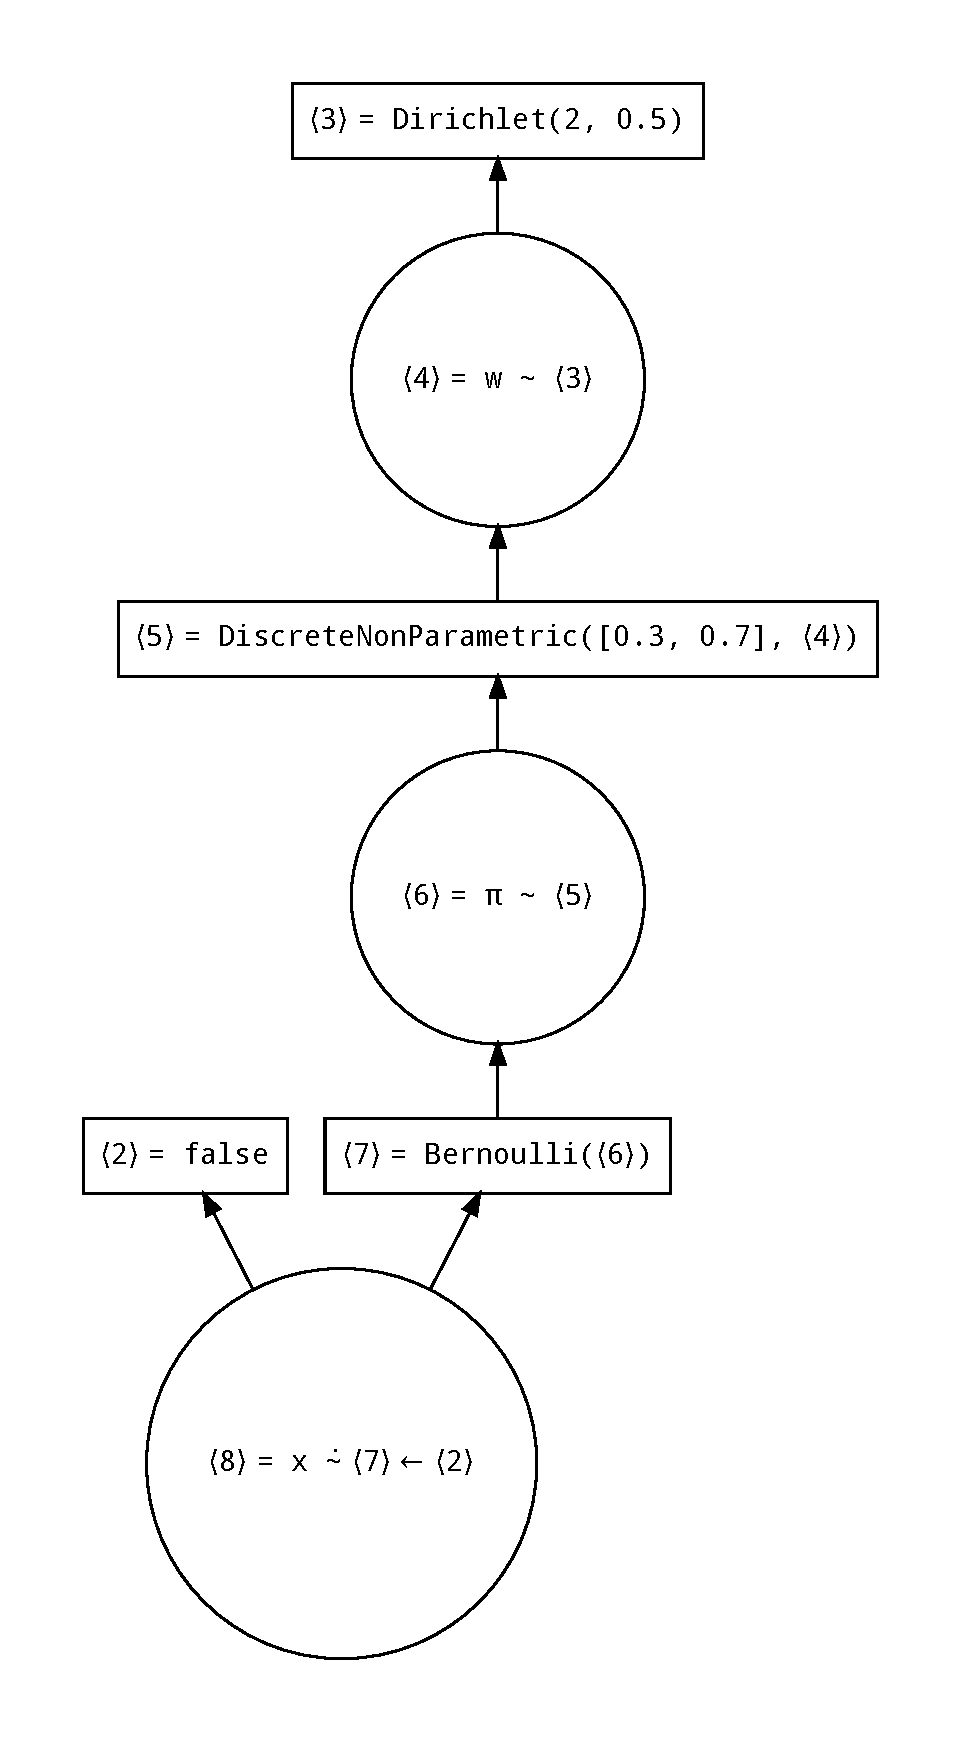
\includegraphics[width=0.49\textwidth]{figures/bernoulli_dependencies}}
  \subbottom[][\texttt{hierarchical\_gaussian(1.4)}]{%
    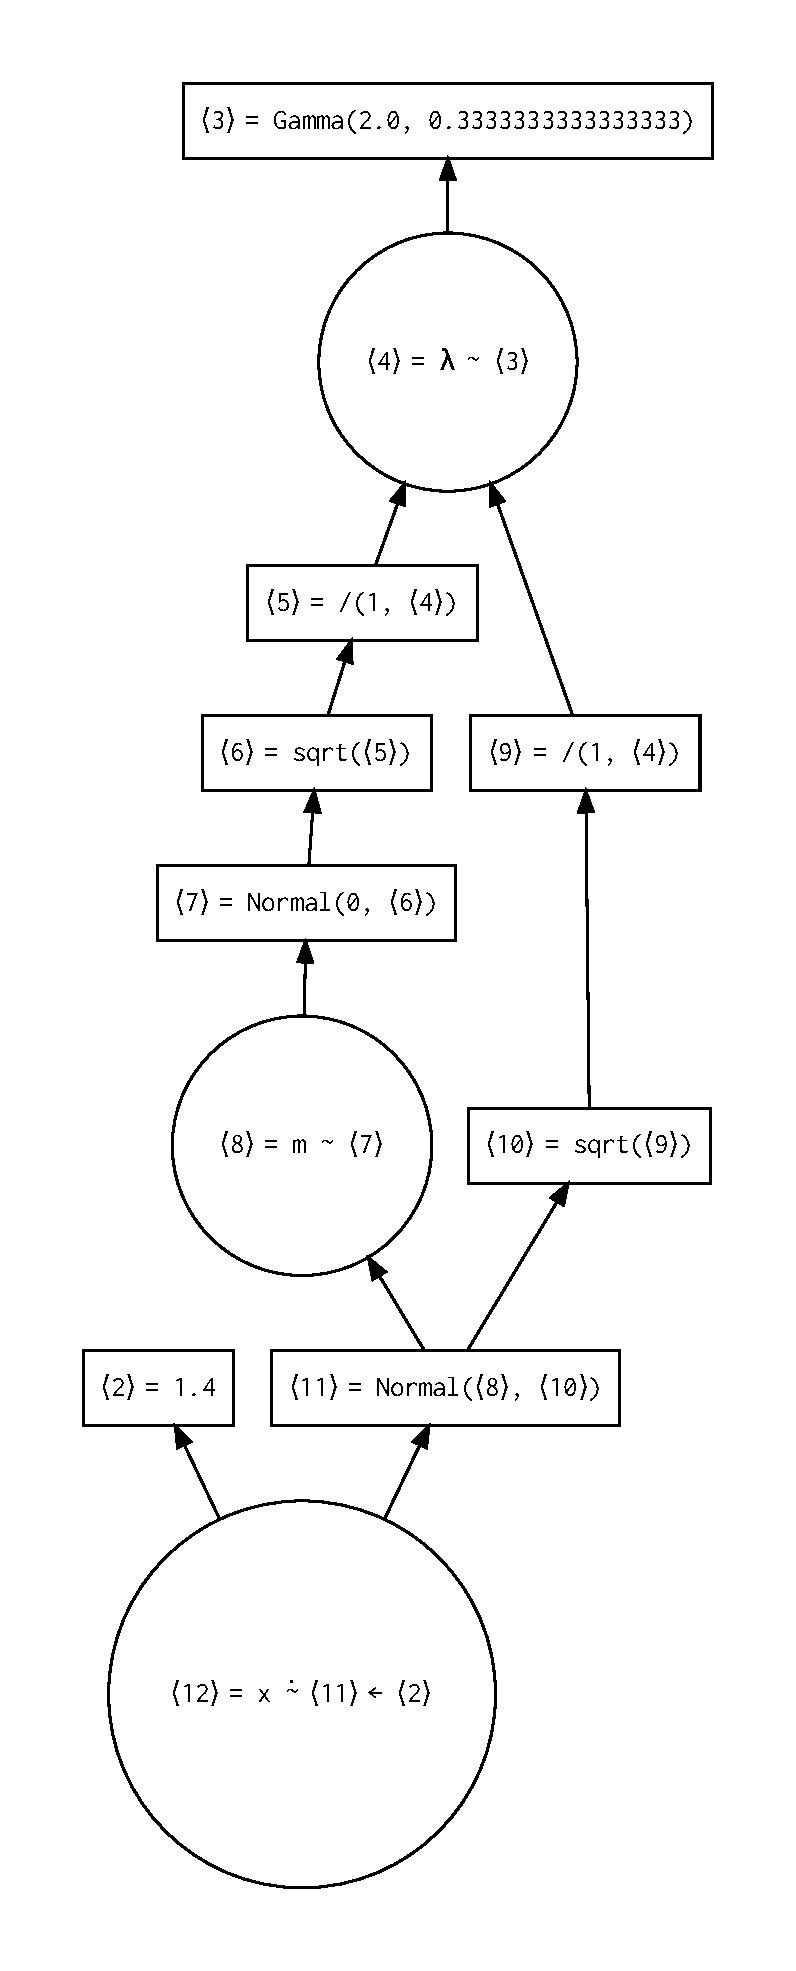
\includegraphics[width=0.49\textwidth]{figures/gaussian_dependencies}}
  \caption{Dependency graphs of the models in listing~\ref{lst:dependency-examples}, generated by
    \autogibbsjl{} and rendered by GraphViz.  More information, such as node values, is stored in
    the real model graph, but not printed for better readability.  Circular nodes denote tilde
    statements, while deterministic intermediate values, corresponding to normal SSA statements, are
    written in rectangles.}
  \label{fig:geom-deps}
\end{figure}


\section{Automatic Calculation of Gibbs Conditionals}
\label{sec:automatic-conditionals}

The ultimate contribution of this work is to utilize the dependency extraction system to extend
\turingjl{} with JAGS-style automatic calculation of Gibbs Conditionals.  In JAGS (and its sibling,
BUGS) conditional extraction works over a wide range of variable types \parencite{plummer2003jags}
by symbolic analysis and recognition of several patterns (e.g., conjugate distributions from
exponential families, log-concave or compactly supported distributions; see
\textcite{lunn2000winbugs}.), which is possible since the class of models is constrained by the
modeling language, and available in completely structured form.

In \turingjl{}, models are much less restricted, and the symbolic form has to recovered from
outside, as we have seen.  To focus on the principal ideas and not to extend the scope too much, the
implementation described in this section was restricted to finite, discrete conditionals, which are
trivial to sample from, given the respective log-density.  Since the construction of conditional
log-densities is independent from the normalization step, though, this can serve as a starting point
for further, more general conditional samplers, as those in JAGS and BUGS.  Additionally, and this
is a more fundamental limitation, the models to which the extraction algorithm can be applied must
be static in a specific sense: the whole Markov blanket of the variable in question must be unique,
and reachable within one run of model tracking.  A large fraction of the models used in practice
do fulfill this condition, though.  As this problem is difficult so solve in general, the same
constraint applies to JAGS and BUGS, which makes \autogibbsjl{} not more limited than these.

The implementation of the conditional extraction system involves three main steps:
\begin{enumerate}
  \firmlist
\item Extracting the symbolic form of the conditional likelihood of Markov blankets in a given
  dependency graph.
\item Constructing closures calculating the normalized discrete conditionals from these likelihoods.
\item Providing a Gibbs-component sampler for \turingjl{}, that can utilize the resulting
  conditional distributions.
\end{enumerate}
The third step turned out to be the easiest, since the sampling system of \turingjl{} is designed to
be extensible.  Ideally, a Gibbs-conditional sampler would have first been added to \turingjl{} and
then simply been reused for \autogibbsjl{}; in practice, it worked out the other way round, and the
\autogibbsjl{} sampler has, in generalized form, been added to \turingjl{} afterwards (without the
automatic extraction, only supporting user-provided conditional distributions).

\newsavebox{\bmlikelihoods}
\begin{lrbox}{\bmlikelihoods}
\begin{lstlisting}[style=lstfloat]
⟨2⟩ = 1.4                  ⤳ 1.4
⟨3⟩ = Dirichlet(2, 0.5)    ⤳ Dirichlet(2, 0.5)
⟨4⟩ = w ~ ⟨3⟩              ⤳ logpdf(Dirichlet(2, 0.5), θ[w])
⟨5⟩ = DNP([0.3, 0.7], ⟨4⟩) ⤳ DNP([0.3, 0.7], θ[w])
⟨6⟩ = π ~ ⟨5⟩              ⤳ logpdf(DNP([0.3, 0.7], θ[w]), θ[π])
⟨7⟩ = Bernoulli(⟨6⟩)       ⤳ Bernoulli(θ[p])
⟨8⟩ = x ~ ⟨7⟩ ← ⟨2⟩       ⤳ logpdf(Bernoulli(θ[p]), θ[x])
\end{lstlisting}
\end{lrbox}
\newsavebox{\hglikelihoods}
\begin{lrbox}{\hglikelihoods}
\begin{lstlisting}[style=lstfloat]
⟨2⟩ = 1.4                 ⤳ 1.4
⟨3⟩ = Gamma(2.0, 1/3)     ⤳ Gamma(2.0, 1/3)
⟨4⟩ = λ ~ ⟨3⟩             ⤳ logpdf(Gamma(2.0, 1/3), θ[λ])
⟨5⟩ = /(1, ⟨4⟩)           ⤳ /(1, θ[λ])
⟨6⟩ = sqrt(⟨5⟩)           ⤳ sqrt(/(1, θ[λ]))
⟨7⟩ = Normal(0, ⟨6⟩)      ⤳ Normal(0, sqrt(/(1, θ[λ])))
⟨8⟩ = m ~ ⟨7⟩             ⤳ logpdf(Normal(0, sqrt(/(1, θ[λ]))), θ[m])
⟨9⟩ = /(1, ⟨4⟩)           ⤳ /(1, θ[λ])
⟨10⟩ = sqrt(⟨9⟩)          ⤳ sqrt(/(1, θ[λ]))
⟨11⟩ = Normal(⟨8⟩, ⟨10⟩)  ⤳ Normal(θ[m], sqrt(/(1, θ[λ])))
⟨12⟩ = x ~ ⟨11⟩ ← ⟨2⟩    ⤳ logpdf(Normal(θ[m], sqrt(/(1, θ[λ]))), θ[x])
\end{lstlisting}
\end{lrbox}
\begin{figure}[t]
  \loosesubcaptions
  \subbottom[\texttt{bernoulli\_mixture(false)}]{\usebox{\bmlikelihoods}}
  \subbottom[\texttt{hierarchical\_gaussian(1.4)}]{\usebox{\hglikelihoods}}
  \caption{Association of the dependency graph of the example models from
    listing~\ref{lst:dependency-examples} with intermediate symbolic functions.  The expressions on
    the right are implicit functions of \protect\jlinl{θ}.  (\texttt{DNP} is used instead of
    \texttt{DiscreteNonParametric} to avoid breaking lines.)}
  \label{fig:continuations}
\end{figure}

Step 1, the symbolic extraction of likelihood functions, is implemented by first converting the full
trace into a symbolic joint log-density.  Therefor the expression of each node in the dependency
graph is associated with a corresponding symbolic representation of a function of the \enquote{trace
  dictionary} \jlinl{θ}, which holds the values of the random variables by name (this is to view the
probabilistic model as a joint distribution over trace dictionaries).  This is done in the following
simple fashion:
\begin{itemize}
  \firmlist
\item References to call nodes or constant nodes (\jlinl{⟨i⟩ = x}) are inlined.
\item References to tilde nodes (\jlinl{⟨j⟩ = v ~ D}) are converted to dictionary lookups: \jlinl{θ[v]}.
\item Call nodes are converted to functions from the trace dictionary to a
  function call on the converted references: \jlinl{f(⟨i⟩, ⟨j⟩)} \(\leadsto\) \jlinl{f(x, θ[v])}.
\item Tilde nodes are converted to log-density evaluations of their values given the corresponding
  distribution: \jlinl{⟨j⟩ = v ~ D} \(\leadsto\) \jlinl{logpdf(D, θ[v])}
\end{itemize}
All resulting expressions are thereby to be understood as implicit functions of \jlinl{θ}.  These
new expression function objects can then be numerically evaluated as log-densities for given values
of all random variables.  For illustration, the joint densities of the \jlinl{bernoulli_mixture} and
\jlinl{hierarchical_gaussian} models introduced above in listing~\ref{lst:dependency-examples}, are
associated with corresponding symbolic functions as shown in figure~\ref{fig:continuations}\todo{fix
  caption alignment}.  By adding the log-likelihoods for each tilde statement, we get the symbolic
log-joint density as, for example,
\begin{lstlisting}
logpdf(Gamma(2.0, 0.333333), θ[λ]) + 
  logpdf(Normal(0, sqrt(/(1, θ[λ]))), θ[m]) + 
  logpdf(Normal(θ[m], sqrt(/(1, θ[λ]))), θ[x]),
\end{lstlisting}
corresponding to the density over \(\lambda\), \(m\), and \(x\), factorized as
\begin{equation}
  p(\lambda, m, x) = p(\lambda) \, p(m \given \lambda) \, p(x \given m, \lambda).
\end{equation}
From this we can then derive conditionals in the usual way of normalizing the proportional
conditional, which can be obtained by removing all terms of the joint factorization that do not
depend on the conditioned variable:
\begin{equation}
  \begin{aligned}
    p(m \given \lambda, x) &\propto p(m \given \lambda) \, p(x \given m, \lambda), \\
    p(\lambda \given m, x) &\propto p(\lambda) \, p(m \given \lambda) \, p(x \given m, \lambda),
  \end{aligned}
\end{equation}
which in more technical terms are given through the \emph{Markov blanket} of \(m\) and \(\lambda\)
\parencites[section 24.2]{murphy2012machine}[section 4.5]{koller2009probabilistic}.

The crucial problem here is, of course, to find the normalization factor, as always in Monte Carlo
methods.  Normalization could, for example, be implemented by analysing the structure of the
resulting expression and detecting conjugacies, such as the normal/normal-gamma relationship between
\(m\), \(\lambda\), and \(x\) above.  The simplest possible case, however, occurs when when a
conditioned variable has finite support; and as mentioned above, this is what has been implemented
out in this work.  For example, \(p\) in the \jlinl{bernoulli_mixture} model is such a finitely
supported variable~-- we get
\begin{equation}
    p(\pi \given w, x) = \frac{p(w) \, p(\pi \given w) \, p(x \given \pi)}{
      \sum_{\varpi \in \{0.3, 0.7\}}p(w) \, p(\varpi \given w) \, p(x \given \varpi)}
\end{equation}
Since the distribution of every variables is preserved in the dependency graph, we now can do the
same thing programmatically, and turn the symbolic log-density into a distribution object by simply
tabulating the values of the denominator through evaluating of the expression over the whole support
of \(\pi\), the set \(\{0.3, 0.7\}\), and summing it up to get the normalization factor.  (This uses
the interface of distribution objects from the \juliapackage{Distributions.jl} package, which have a
\jlinl{support} method whose result is an iterable.)

Concretely, the construction works as follows, finalizing step 2 of the above scheme, exemplified by
\jlinl{bernoulli_mixture}:
\begin{enumerate}
  \firmlist
\item Find the likelihood expressions that match a given conditioned variable (this includes indexed
  variables subsumed by a parent, like \jlinl{v[i]} and \jlinl{v}), and their distribution:
  \begin{equation*}
    \begin{aligned}
      \ell_{1} &= \mathtt{logpdf(DNP([0.3, 0.7],\theta[w]), \theta[\pi])}. \\
      \mathcal{D} &= \mathtt{DNP([0.3, 0.7], \theta[w])}.
    \end{aligned}
  \end{equation*}
\item For each of these (sub-)variables, collect the likelihoods of their children variables, thus
  completing the Markov blanket:
  \begin{equation*}
    \ell_{2} = \mathtt{logpdf(Bernoulli(\theta[\pi]), \theta[x])}
  \end{equation*}
  The complicated part of this and the previous step is the correct matching of indexed variables in
  the trace dictionary: forms like \jlinl{θ[v][1]} and \jlinl{θ[v[1]]} need to be resolved correctly
  to the same value.
\item Construct for each a closure function that takes as an argument a fixed trace dictionary,
  tabulates the conditional log-likelihood over it with the conditioned variable fixed to all values
  of its support, and normalizes the result:\todo{Better typesetting?}
  \begin{equation*}
    \begin{aligned}
      &\theta \mapsto \{ \\
      &\quad \Omega = \mathtt{support}(\mathcal{D}) \\
      &\quad \mathtt{table} = \left[\operatorname{eval}(\ell_{1}, \theta[\pi \leadsto \varpi]) +
        \operatorname{eval}(\ell_{2}, \theta[\pi \leadsto \varpi]) \mid \varpi \in \Omega \right] \\
      &\quad \distr{DNP}(\Omega, \operatorname{softmax}(\mathtt{table})) \\
      &\}
    \end{aligned}
  \end{equation*}
  (whereby \(\operatorname{softmax}(x) = \broadcast{\exp}(x) / \sum_i \exp(x_{i})\) is the
  normalization operation on log-probabilities).
\end{enumerate}
The result of this process is a collection of closures that represent the conditional likelihoods as
\enquote{kernels}: functions from conditioned-on variables to distribution objects.  These closures
can then be used to construct a conditional sampler for usage in \turingjl{}'s \jlinl{Gibbs}
sampler, in combination with other samplers for the continuous variables.

\newthought{As for potential improvements}, there is of course a wide range of possibilities, as the
current implementation is a most primitive one.  As has been mentioned before, further classes of
random variables beyond those with finite support could be handled, using methods and heuristics as
in BUGS or JAGS.  This could even involve symbolic methods like those in AutoConj
\parencite{hoffman2018autoconj}. More generally, variance-reducing transformation, as those in
\textcite{murray2017delayed}, are applicable.  For computational efficiency, a parallel Gibbs
sampler \parencite{gonzalez2011parallel} could be constructed, improving scalability with increasing
data size (i.e., numbers of observations).  Or, as in \juliapackage{Gen.jl}, a variant of
\enquote{argument diffs} could be devised to prevent unnecessary re-evaluation of model parts
\parencites[see][section 1.2.3]{cusumano-towner2020gen}{becker2020dynamic}.

Besides improvements via inference algorithms, it would be possible for models that are written in a
vectorized or otherwise \enquote{trace constant} fashion, such that the structure of the
conditionals does not change with the number of observations, to record the trace for a small model
and reuse it for arbitrary larger ones, thus avoiding recomputation and recompilation.  Finally, the
evaluation of the conditional closures, which is currently performed by simple interpretation of
expressions, could be sped up by compiling them to Julia methods, or even better by reusing the
SSA-like structure to emit Julia IR directly.

Realistically, though, I consider it more worthwhile to follow a different approach, like the one
outlined in section~\ref{sec:future-work} below, and moving away from working on a trace-based
reconstruction and to a domain-specific intermediate representation with generalized transformation
capabilities.  On such a representation, all of the named ideas still apply, but it would have the
advantage of being more invariant to a specific inference system, and be able to handle more general
probabilistic programs (foremost, not only static ones).


\section{Evaluation}
\label{sec:autogibbs-eval}

To begin with a qualitative assessment, it must be admitted that \autogibbsjl{} is, when run
manually and only once, empirically so noticeably slow, that a user may be tempted to dismiss it
outright (concretely speaking, extraction of one conditional for some not-so-large models takes
\(20\) to \(200\) seconds on the author's laptop).  This is a valid point, but two counter-arguments
must be considered.  For one, the implementation is a preliminary one, more conceptual than
optimized.  Much of the slow-down could be mitigated by just improving key parts of \autogibbsjl{}
and \irtrackerjl{}.

In addition to that, one must realize where this apparent slowness comes from: namely, from
compilation, and therein primarily type inference, of the functions handling all the strongly typed
expression trees.  Besides the possibility of just optimizing these further, the following fact is
most important to realize: compilation takes place only once~-- as soon as a conditional is
constructed, it can be reused in arbitrarily many sampling runs of the same model.  The finished
conditionals then do not take so much time anymore, quite the contrary: they are much faster than
other within-Gibbs samplers, since they only involve evaluating a fixed expression, constructing a
distribution, and sampling from it once (and even this could be sped up further).  This makes it
possible to sample much longer chains in the same time, which is an overall advantage.

Furthermore, due to the limitations \autogibbsjl{} puts on the structure of variable names, there
are cases in which models cannot be formulated in a certain desirable way in \dppljl{}, thus losing
certain advantages such as block-wise treatment of collections of independent variables.  This can
lead to a disadvantage compared to other samplers.  Again, the restrictions are mostly a detail of
the current implementation, and there is no theoretical hindrance in overcoming than.

So, to conclude, while the implementation in current form is not applicable in practice for all
possible cases, it is very much so in principle.  Based on the lessons learned through this work,
further contributions to Gibbs sampling in \turingjl{} are already planned (although not necessarily
based on \autogibbsjl{}).

\newthought{For a more {q}uantitative} point of view, let us now turn to some empirical evaluations.
Besides several unit tests for correctness of the derived dependencies and conditionals on a variety
of small models chosen to test certain features and corner cases, an experimental comparison of
\autogibbsjl{} and existing \turingjl{} samplers has been conducted.  Three off-the-shelf Bayesian
models were chosen: a Gaussian mixture model (GMM) with known variances and priors over cluster
centers, weights, and assignments \parencite[section 6.2]{marin2007bayesian}:
\begin{equation}
  \label{eq:gmm}
  \begin{aligned}
    w &\from \distr{Dirichlet(K)} \\
    z_{n} &\from \distr{Categorical}([1, \ldots, K], w), \quad n = 1, \ldots, N \\
    \mu_{k} &\from \Normal(0, \sigma_{1}), \quad k = 1, \ldots, K \\
    x_{n} &\from \Normal(\mu_{z_{n}}, \sigma_{1}), \quad n = 1, \ldots, N;
  \end{aligned}
\end{equation}
a hidden Markov model
(HMM) with known variances and priors over transition and emission probabilities \parencite[section
7.3]{marin2007bayesian}:
\begin{equation}
  \label{eq:hmm}
  \begin{aligned}
    T_{k} &\from \distr{Dirichlet}(K), \quad k = 1, \ldots, K \\
    m_{k} &\from \Normal(k, \sigma_{1}), \quad k = 1, \ldots, K \\
    s_{1} &\from \distr{Categorical}([1, \ldots, K], [1/K, \ldots, 1/K]) \\
    s_{k} &\from \distr{Categorical}([1, \ldots, K], T_{s_{k-1}}), \quad k = 2, \ldots, N \\
    x_{k} &\from \Normal(m_{s_{k}}, \sigma_{2}), \quad k = 1, \ldots, N;
  \end{aligned}
\end{equation}
and an infinite mixture model (IMM) in stick-breaking construction, but
otherwise of the same form as the GMM, to represent a nonparametric example \parencite[section
2.2]{hjort2010bayesian}:
\begin{equation}
  \label{eq:imm}
  \begin{aligned}
    w &\from \distr{TruncatedStickBreakingProcess(\alpha, K)} \\
    z_{n} &\from \distr{Categorical}([1, \ldots, K], w), \quad n = 1, \ldots, N \\
    \mu_{k} &\from \Normal(0, \sigma_{1}), \quad k = 1, \ldots, K \\
    y_{n} &\from \Normal(\mu_{z_{n}}, \sigma_{2}), \quad n = 1, \ldots, N.
  \end{aligned}
\end{equation}
In the context of this work, the three interesting classes of metrics are
\begin{enumerate}
  \firmlist
\item the \enquote{extraction time} of \autogibbsjl{}, i.e., the time it takes to extract and a
  conditional including compilation times,
\item the sampling speed when used as component of a within-Gibbs sampler, and
\item the quality of the resulting chains, in terms of convergence and variance diagnostics.
  (Although this really measures Gibbs sampling, not the implementation of \autogibbsjl{}, it is a
  relevant comparison for the practitioner.)
\end{enumerate}
To estimate them, a series of experiments has been conducted.  Each of the test models involves one
discrete and two continuous parameter arrays.  As a baseline for \autogibbsjl{}'s static conditional
(AG), \turingjl{}'s Particle Gibbs sampler (PG) was chosen, which is also suited to discrete
parameters.  PG was always used with \(100\) particles, since lower values did not lead to
convergent chains.  Continuous variables were all sampled using Hamiltonian Monte Carlo (HMC) with
hand-tuned parameters (\(10\) leapfrog steps with step size \(0.05\)).  The experiments have been
set up to vary between AG and PG, and between \(10\), \(25\), and \(50\) observations, since their
number determines the size of the trace, and thus influences both AG's compile times and the overall
sampling time.  All measurements were conducted using the following system configuration, as shown
by \jlinl{InteractiveUtils.versioninfo()}:
\begin{lstlisting}
Julia Version 1.3.1
Commit 2d5741174c (2019-12-30 21:36 UTC)
Platform Info:
  OS: Linux (x86_64-pc-linux-gnu)
  CPU: Intel(R) Core(TM) i5-4690 CPU @ 3.50GHz
  WORD_SIZE: 64
  LIBM: libopenlibm
  LLVM: libLLVM-6.0.1 (ORCJIT, haswell)
\end{lstlisting}
Everything was executed single-threaded, with exclusive resource access on the server, to preclude
measurement noise as much as possible.  Each of the three models was benchmarked in a separate Julia
session.  The last two chains of the HMM with \(50\) observations using Particle Gibbs could not be
completed, due to the twelve hour time limit set by the job scheduler.  The raw data can be found in
\textcite{gabler2020mcmc}. 

The \dppljl{} implementations of the models can be found in listing~\ref{lst:evaluation-models}.
Note that for each, there exists a second, equivalent implementation used for PG, since particle
samplers in \turingjl{} require the usage of special data types due to their task copying mechanism.

\newthought{It follows} a detailed analysis of the results per model in graphical form, based on six
plots each.  First, PG and AG are compared in terms of sampling times by number of observations on
the top left.  Right of this, we have the dependency of the extraction time of AG given the number
observations.  The first of these points is almost always an outlier, since it involves additional
compilation time.  Through the rest, a quadratic function is fitted, which always matched the values
very closely.

On the recto pages, plots for convergence analysis are visualized.  Since these are estimated per
parameter, and the test models involve larger arrays of parameters, the first elements of the
continuous and the fifth element of the discrete parameters have always been chosen as
representatives.  On the top, the first chain of each experimental combination is shown as a
qualitative representative (thinned for ease of plotting).  Well-converging chains should look like
white noise, not like a random walk.  In the middle plot, the estimated autocorrelation functions of
the same chains are given, which are a way to evaluate convergence speed by eye.  The functions
should vanish quickly (indicated by the gray significance bar around the abscissa); uncorrelated
samples would have zero autocorrelation except for the first lag.

Lastly, two diagnostic values are plotted for each combination and chain.  The
\enquote{scale-reduction} \(\widehat{\mathrm{R}}\), after \textcite{gelman1992inference}, estimates
the factor by which the scale of the current distribution might be reduced if the simulations were
continued \parencite[see][p. 285]{gelman2020bayesian}.  It should be close to one for indicating
good convergence; as a rule of thumb, a value of more than \(1.1\) is suspicious.  The effective
sample size (ESS) arises in the estimation of the asymptotic variance of Markov chains
\parencite[][section 7.2]{vihola2020lectures}, where it is formally analogous to the sample size in
the variance estimator for \iid{} variables.  The ESS can also be interpreted as a one-point summary
of the autocorrelation estimate, normalized by chain length.  It should be close to the actual
number of samples, or at least of the same order of magnitude.

%%%%%%%%%%%%%%%%%%%%%%%%%%%%%%%%%%%%%%%%%%%%%%%%%%%%%%%%%%%%%%%%%%

\begin{lstfloat}[p]
\begin{lstlisting}[style=lstfloat]
@model function gmm(x, K)
    N = length(x)
    w ~ Dirichlet(K, 1/K)  # Cluster association prior
    z ~ filldist(Categorical(w), N)  # Cluster assignments
    μ ~ filldist(Normal(0.0, s1_gmm), K)  # Cluster centers

    for n = 1:N
        x[n] ~ Normal(μ[z[n]], s2_gmm)  # Observations
    end
end

@model function hmm(x, K, ::Type{T}=Float64) where {T<:Real}
    N = length(x)

    T = Vector{Vector{X}}(undef, K)
    for i = 1:K
        T[i] ~ Dirichlet(K, 1/K)  # Transition probabilities
    end
    
    s = zeros(Int, N)
    s[1] ~ Categorical(K)
    for i = 2:N
        s[i] ~ Categorical(T[s[i-1]])  # State sequence
    end
    
    m = Vector{T}(undef, K)
    for i = 1:K
        m[i] ~ Normal(i, s1_hmm)  # Emission probabilities
    end
    
    x[1] ~ Normal(m[s[1]], s2_hmm)
    for i = 2:N
        x[i] ~ Normal(m[s[i]], s2_hmm)  # Observations
    end
end

@model function imm_stick(y, α, K)
    N = length(y)
    crm = DirichletProcess(α)
    v ~ filldist(StickBreakingProcess(crm), K - 1)
    w = stickbreak(v)  # Cluster weights
    
    z = zeros(Int, N)
    for n = 1:N
        z[n] ~ Categorical(w)  # Cluster assignments
    end

    μ ~ filldist(Normal(0.0, s1_imm), K)  # Cluster centers

    for n = 1:N
        y[n] ~ Normal(μ[z[n]], s2_imm)  # Observations
    end
end
\end{lstlisting}
  \caption{Gaussian mixture model, hidden Markov model, and infinite mixture model using a
    stick-breaking construction.  The two-step calculation of \texttt{w} via \texttt{v} is a
    technicality due to \turingjl{}'s handling of nonparametric models.  The function
    \texttt{stickbreak} normalizes the stick-lengths \texttt{v} into a Dirichlet-like distribution.
    The \texttt{Categorical(p)} constructor automatically infers the support of the categorical
    distribution from the weight vector as \texttt{1:length(p)}.}
  \label{lst:evaluation-models}
\end{lstfloat}

%%%%%%%%%%%%%%%%%%%%%%%%%%%%%%%%%%%%%%%%%%%%%%%%%%%%%%%%%%%%%%%%%%
\cleartoverso
\FloatBlock

\newcommand{\leftplotcaption}[1]{%
  Sampling and extraction times for #1, factored by algorithm and number
  of observations.  Points are jittered horizontally to increase readability.  A quadratic curve is
  fitted to the extraction times.
}
\newcommand{\rightplotcaption}[1]{%
  Diagnostics, factored by algorithm, number of observations, and a selection of model parameters.
  \(\widehat{\mathrm{R}}\) and ESS point estimates are jittered horizontally for better readability.
  For chain plots and autocorrelation, the first chain of the respective combination has been used.
}

\begin{figure}[t!]
  \centering
  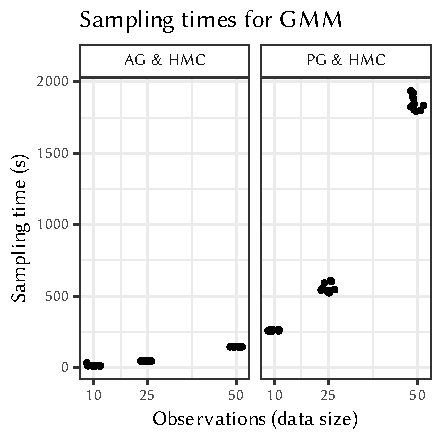
\includegraphics[width=0.49\textwidth]{figures/GMM-sampling_times}
  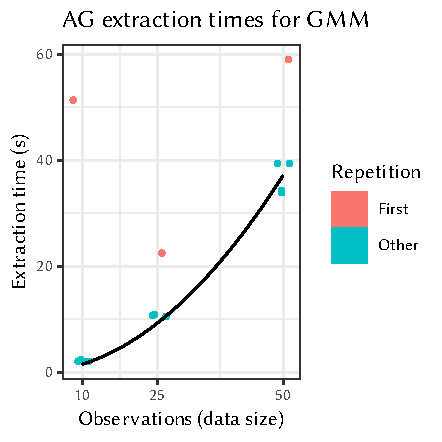
\includegraphics[width=0.49\textwidth]{figures/GMM-compile_times}
  \caption{\leftplotcaption{GMM}}
  \label{fig:plots-gmm}
\end{figure}

\subsection*{Gaussian Mixture Model}

For the GMM, the AG sampling times lie consistenly below the minimum of the PG sampling times, even
with the largest number of observations.  Extraction time seems to grow quadratically, with
exception of the first call of the conditional extraction, involving compilation and type
inference.

The mixing behaviour of the chains shows a large variation.  With \(10\) and \(25\) observations,
neither of the altgorithms reaches consistently satisfactory results; the distribution of
\(\widehat{R}\) values is quite diffuse and suspiciously large (more so for PG), and especially the
ESS numbers are way too low.  A look at the exemplary autocorrelation plots seems to confirm bad
convergence.  The corresponding chains clearly show random-walk-like or \enquote{lumped} behaviour
for some combinations.

For \(50\) observations, the result is different with AG.  The \(w\) and \(\mu\) parameters appear
to converge well in most cases, with very low-variance chains and visibly large ESS values.  But for
unknown reasons, the \(z\) parameter seems to have gotten \enquote{stuck} in this particular example
and not moved at all, which is the reason no autocorrelation function could be estimated.  PG might
have improved somewhat, looking at the lower \(\widehat{R}\) distributions, but not enough to make a
meaningful difference, as ESS and autocorrelation plots show no sufficiently good behaviour.


\cleartorecto
\FloatBlock

\begin{figure}[p]
  \centering
  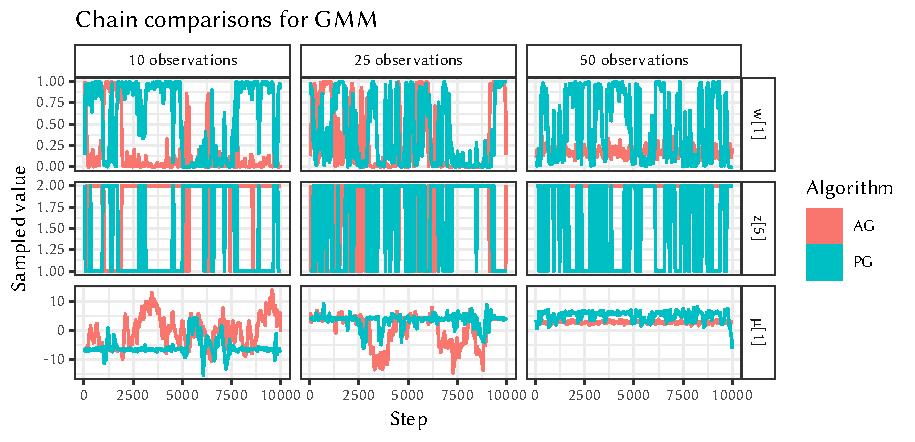
\includegraphics[width=\textwidth]{figures/GMM-chains}
  \par
  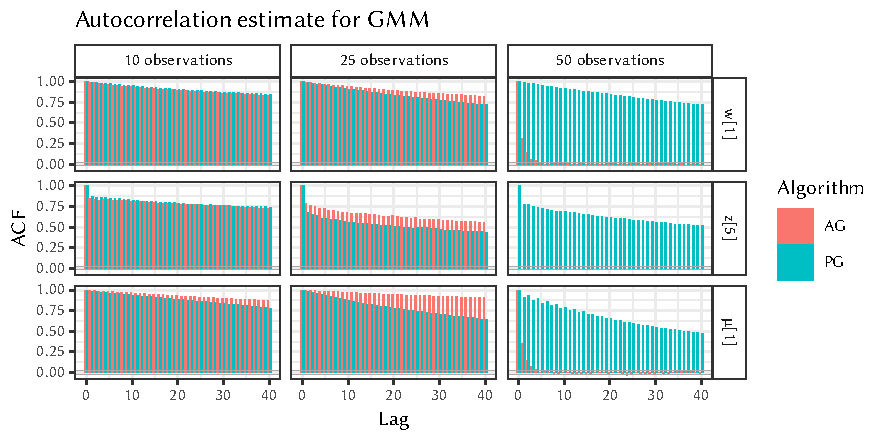
\includegraphics[width=\textwidth]{figures/GMM-acfs}
  \par
  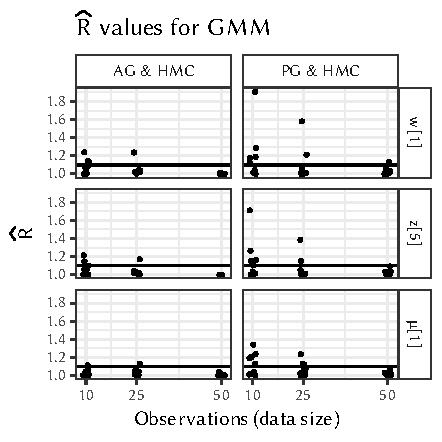
\includegraphics[width=0.49\textwidth]{figures/GMM-rhat}
  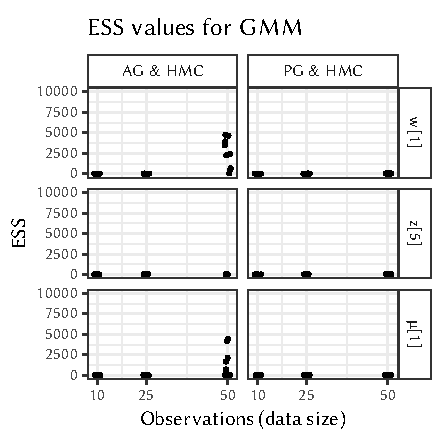
\includegraphics[width=0.49\textwidth]{figures/GMM-ess}
  \contcaption{\rightplotcaption{GMM}}
\end{figure}

%%%%%%%%%%%%%%%%%%%%%%%%%%%%%%%%%%%%%%%%%%%%%%%%%%%%%%%%%%%%%%%%%%
\cleartoverso
\FloatBlock

\begin{figure}[t!]
  \centering
    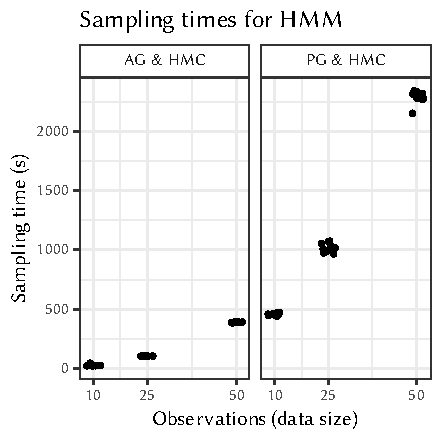
\includegraphics[width=0.49\textwidth]{figures/HMM-sampling_times}
  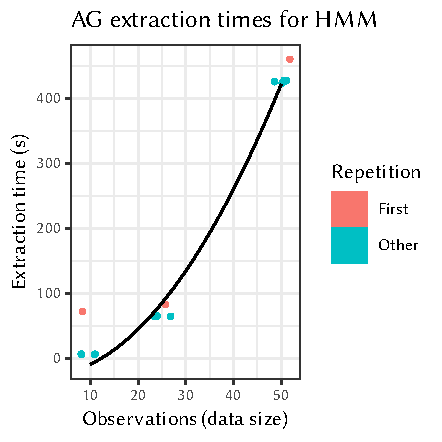
\includegraphics[width=0.49\textwidth]{figures/HMM-compile_times}
  \caption{\leftplotcaption{HMM}}
  \label{fig:plots-hmm}
\end{figure}

\subsection*{Hidden Markov Model}

Also for HMM, the same trends in sampling and extraction times as with GMM are visible, with AG
being consistenly faster.  The extraction times seem to be quite the same as GMM, even in absolute
terms, as are the outliers of the first function calls.

Mixing behaviour for this model is much better overall.  The chains look less like random walks,
especially for \(\mu\).  Autocorrelation plots are sometimes quite good, especially for \(s\), and
in all cases better as those above for GMM.  The \(\widehat{R}\) values are all in better ranges
(note the difference in the scale of the ordinate!), and ESS noticeably higher.  Overall, AG seems
to improve over PG on average, although neither of the results is stellar.

\cleartorecto
\FloatBlock

\begin{figure}[p]
  \centering
  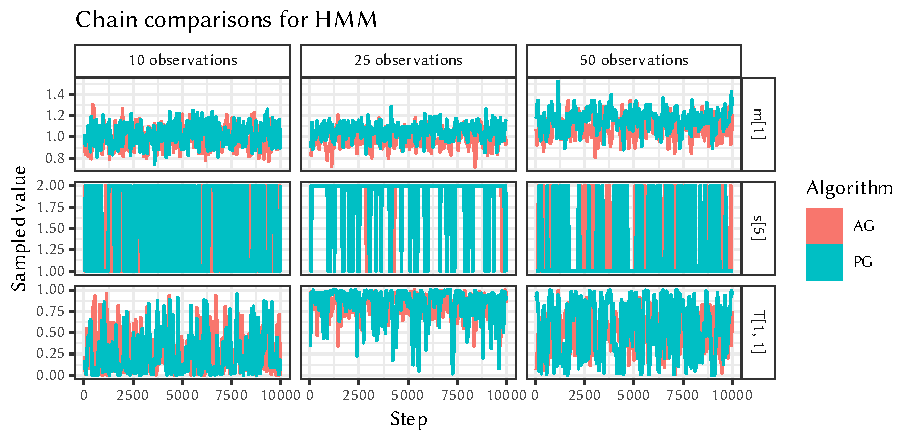
\includegraphics[width=\textwidth]{figures/HMM-chains}
  \par
  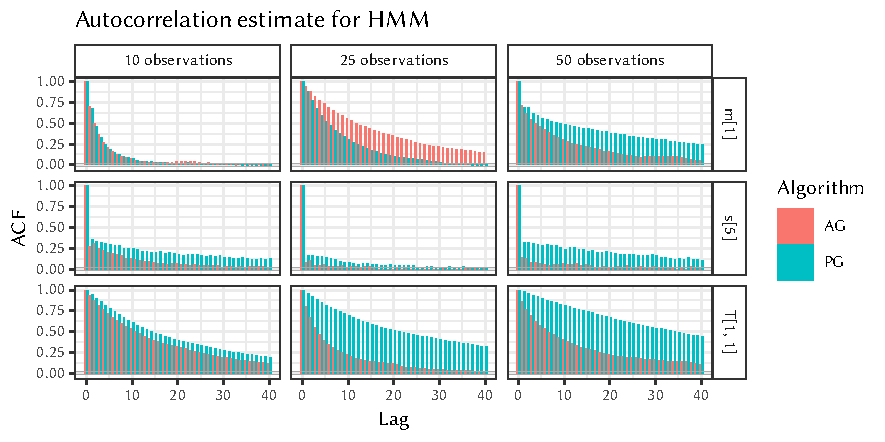
\includegraphics[width=\textwidth]{figures/HMM-acfs}
  \par
  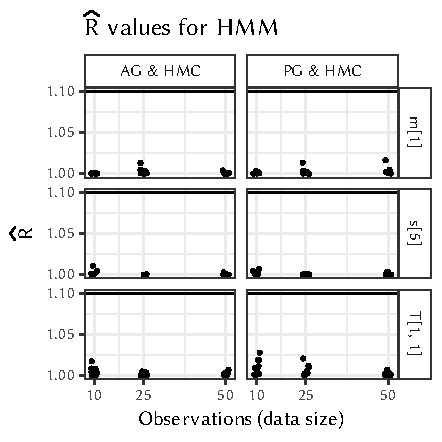
\includegraphics[width=0.49\textwidth]{figures/HMM-rhat}
  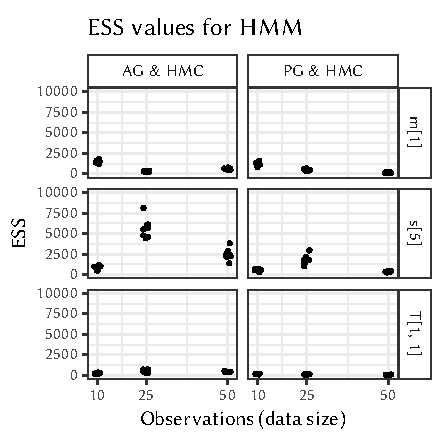
\includegraphics[width=0.49\textwidth]{figures/HMM-ess}
  \contcaption{\rightplotcaption{HMM}}
\end{figure}

%%%%%%%%%%%%%%%%%%%%%%%%%%%%%%%%%%%%%%%%%%%%%%%%%%%%%%%%%%%%%%%%%%
\cleartoverso
\FloatBlock

\begin{figure}[t!]
  \centering
  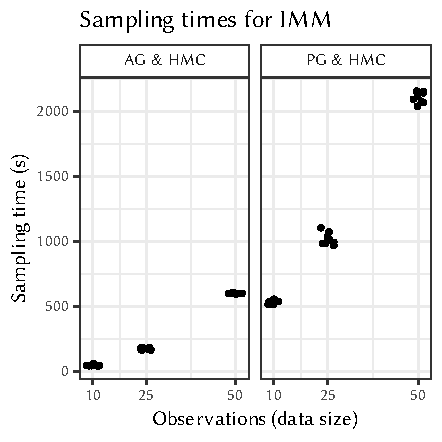
\includegraphics[width=0.49\textwidth]{figures/IMM-sampling_times}
  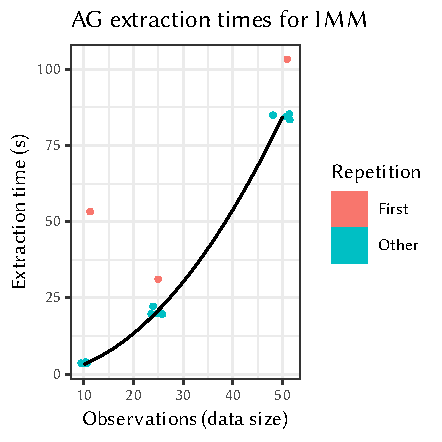
\includegraphics[width=0.49\textwidth]{figures/IMM-compile_times}
  \caption{\leftplotcaption{IMM}}
  \label{fig:plots-imm}
\end{figure}

\subsection*{Infinite Mixture Model}

Again, similar trends of sampling times and extraction times are noticeable.  Here we can observe
some larger involved factors, though; both curves grow faster, with PG on \(10\) observations even
being faster than AG on \(50\) observations; although still on a significantly higher scale in
general.

In this example, PG appears to work better on average.  In the example chain plots, we can only see
a noticeable difference for \(\mu\), while the autocorrelation graphs are almost all worse for AG
(although both algorithms seem to do better than in the GMM test).  ESS is only satisfactory for the
\(z\) parameters, but PG here shows a much more consistent behaviour of the \(\widehat{R}\)
distribution.


\begin{figure}[p]
  \centering
  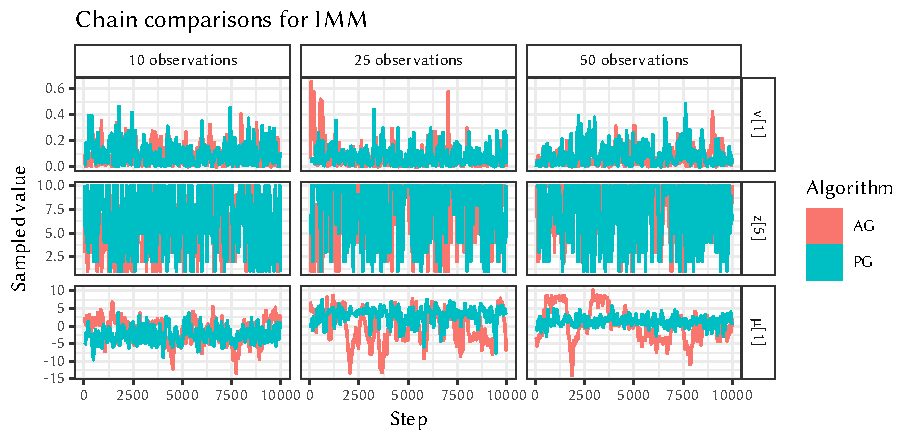
\includegraphics[width=\textwidth]{figures/IMM-chains}
  \par
  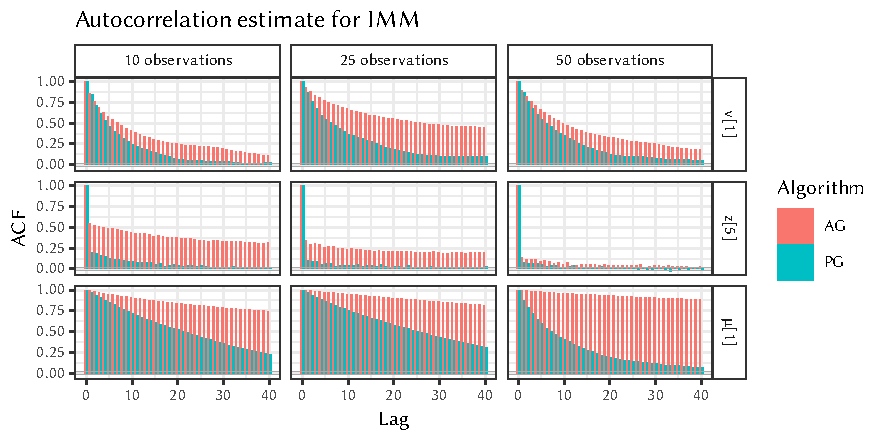
\includegraphics[width=\textwidth]{figures/IMM-acfs}
  \par
  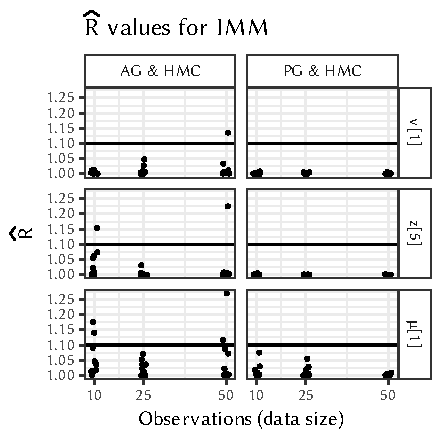
\includegraphics[width=0.49\textwidth]{figures/IMM-rhat}
  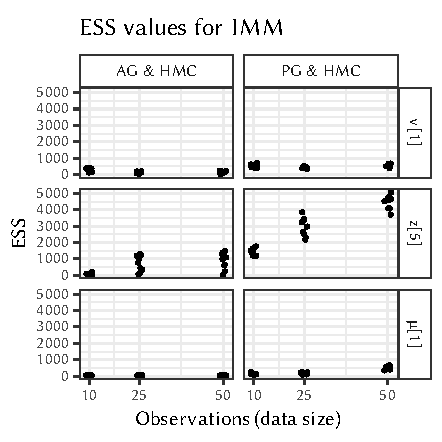
\includegraphics[width=0.49\textwidth]{figures/IMM-ess}
  \contcaption{\rightplotcaption{IMM}}
\end{figure}

\FloatBlock


\subsection*{Summary}

Whereas the sampling times of Particle Gibbs always grows rather fast, depending on the number of
observations, the rate of growth seems to be much lower for AutoGibbs.  The behaviour of these
curves appears to be superlinear, perhaps quadratic.  For GMM and HMM, the maximal sampling time of
AG is always below the minimal sampling time of PG.  Even in the case of IMM, AG's sampling time
with \(50\) observations is closest to PG's with only \(10\) particles, with the latter still
obviously rising much faster.

With regard to the extraction times, we can note a pretty clear quadratic run time depending on the
number of observations.  The first run is always significantly above this trend, due to the impact
of compilation and type inference.  Additionally, the first invocation for the lowest number of
observations might have involved additional compilation of library functions, explaining the larger
residual compared to the first runs of the larger numbers.

In terms of convergence, AG and PG deliver quite comparable results, varying with some variation in
quality depending on model and number of observations.  In most cases, judging by eye through the
exemplary autocorrelation plots, one or the other seems to slightly beat the other, which is
buttressed by the distribution of the diagnostic values.  IMM seems poses a particularly bad
application for AG, but otherwise, no consistent \enquote{winner} is visible, and variations do not
seem to follow a consistent pattern.

In conclusion, it can be said that for models where both are applicable, AutoGibbs provides a viable
alternative to PG, delivering comparable results in less time.  Care has to be taken to diagnose
mixing behaviour, though, as always in MCMC simulations.


% \begin{table}[t]
%   \centering
%   \libertineTabular
%   \begin{tabularx}{\textwidth}{XXrrr@{\hskip 10mm}rrrr}
%     \toprule
%      & & \multicolumn{3}{c@{\hskip 10mm}}{\textbf{GMM}} & \multicolumn{3}{c}{\textbf{HMM}} & \multicolumn{1}{c}{\textbf{IMM}} \\
%     \midrule
%     & HMC Step size & & 0.05 & & & 0.05 & & 0.05 \\
%     & HMC Steps & & 10 & & & 10 & & 10 \\
%     \midrule
%     \textbf{AG + HMC} & Observations & 10 & 25 & 50 & 10 & 25 & 50 & 10 \\
%     & Chains & 30 & 30 & 30 & 30 & 30 & 30 & 30 \\
%     & Compilations & 3 & 3 & 3 & 3 & 3 & 3 & 3 \\
%     \addlinespace
%     \textbf{PG + HMC,} & Observations & 10 & 25 & 50 & 10 & 25 & 50 & 10 \\
%      & Chains & 10 & 10 & 10 & 10 & 10 & 10 & 10 \\
%     \bottomrule
%   \end{tabularx}
%   \caption{Experimental conditions for evaluating AutoGibbs (AG) against Particle Gibbs (PG).  Chains
%     were always of length \(10000\).  A new static Gibbs conditional was extracted for each block of
%     \(10\) chains that was run with the same parameters while Particle Gibbs was varied over the
%     three particle sizes.  Particle Gibbs with 50 particles was sometimes killed due to timeouts on
%     the server.}
%   \label{tab:autogibbs-params}
% \end{table}



% extraction times
% Measuring both compilation of the traced code and the conditional calculation.",
% "All 2 or 3 repetitions per data size class are shown."
% Linear fit for time ~ datasize²
% three samples

% sampling times
% subtitle = "Factored by algorithm and number of PG particles"

% diagnostics
% subtitle = "Factored by algorithm and number of particles"

% densities
% subtitle = paste("Factored by number of observations (data size)", "and selected parameters")

% ACFs
% subtitle = "ACF plots for one sample chain per data size"


%%% Local Variables: 
%%% TeX-master: "main"
%%% End: